% Options for packages loaded elsewhere
\PassOptionsToPackage{unicode}{hyperref}
\PassOptionsToPackage{hyphens}{url}
%
\documentclass[
  11pt,
]{article}
\usepackage{amsmath,amssymb}
\usepackage{lmodern}
\usepackage{ifxetex,ifluatex}
\ifnum 0\ifxetex 1\fi\ifluatex 1\fi=0 % if pdftex
  \usepackage[T1]{fontenc}
  \usepackage[utf8]{inputenc}
  \usepackage{textcomp} % provide euro and other symbols
\else % if luatex or xetex
  \usepackage{unicode-math}
  \defaultfontfeatures{Scale=MatchLowercase}
  \defaultfontfeatures[\rmfamily]{Ligatures=TeX,Scale=1}
  \setmainfont[]{Georgia}
  \setsansfont[]{PT Sans Caption}
\fi
% Use upquote if available, for straight quotes in verbatim environments
\IfFileExists{upquote.sty}{\usepackage{upquote}}{}
\IfFileExists{microtype.sty}{% use microtype if available
  \usepackage[]{microtype}
  \UseMicrotypeSet[protrusion]{basicmath} % disable protrusion for tt fonts
}{}
\makeatletter
\@ifundefined{KOMAClassName}{% if non-KOMA class
  \IfFileExists{parskip.sty}{%
    \usepackage{parskip}
  }{% else
    \setlength{\parindent}{0pt}
    \setlength{\parskip}{6pt plus 2pt minus 1pt}}
}{% if KOMA class
  \KOMAoptions{parskip=half}}
\makeatother
\usepackage{xcolor}
\IfFileExists{xurl.sty}{\usepackage{xurl}}{} % add URL line breaks if available
\IfFileExists{bookmark.sty}{\usepackage{bookmark}}{\usepackage{hyperref}}
\hypersetup{
  pdftitle={PMBCL survival analysis},
  pdfauthor={Cornelius Hennch},
  hidelinks,
  pdfcreator={LaTeX via pandoc}}
\urlstyle{same} % disable monospaced font for URLs
\usepackage[margin=1in]{geometry}
\usepackage{graphicx}
\makeatletter
\def\maxwidth{\ifdim\Gin@nat@width>\linewidth\linewidth\else\Gin@nat@width\fi}
\def\maxheight{\ifdim\Gin@nat@height>\textheight\textheight\else\Gin@nat@height\fi}
\makeatother
% Scale images if necessary, so that they will not overflow the page
% margins by default, and it is still possible to overwrite the defaults
% using explicit options in \includegraphics[width, height, ...]{}
\setkeys{Gin}{width=\maxwidth,height=\maxheight,keepaspectratio}
% Set default figure placement to htbp
\makeatletter
\def\fps@figure{htbp}
\makeatother
\setlength{\emergencystretch}{3em} % prevent overfull lines
\providecommand{\tightlist}{%
  \setlength{\itemsep}{0pt}\setlength{\parskip}{0pt}}
\setcounter{secnumdepth}{5}
\usepackage{longtable}
\usepackage{booktabs}
\LTcapwidth=.95\textwidth
\linespread{1.05}
\usepackage{hyperref}
\usepackage{array}
\usepackage{multirow}
\usepackage{wrapfig}
\usepackage{float}
\usepackage{colortbl}
\usepackage{pdflscape}
\usepackage{tabu}
\usepackage{threeparttable}
\usepackage{threeparttablex}
\usepackage[normalem]{ulem}
\usepackage{makecell}
\usepackage{xcolor}
\ifluatex
  \usepackage{selnolig}  % disable illegal ligatures
\fi

\title{PMBCL survival analysis}
\author{Cornelius Hennch}
\date{18.06.2021}

\begin{document}
\maketitle

\hypertarget{cohort-overview}{%
\section{Cohort overview}\label{cohort-overview}}

\textbf{Comment:} I created this document to learn how to create
Rmarkdown documents. I won't continue working with the Rmarkdown
notebook document, as re-runs all the code, which makes it too time
consuming at some point. My main take-aways from writing this script
were the following:

\begin{enumerate}
\def\labelenumi{\arabic{enumi}.}
\tightlist
\item
  Setting the correct working directory for knitting is important and a
  little bit counter-intuitive (use \texttt{rmarkdown::render} rather
  than the Knit button).
\item
  If set-up correctly, the same document can be knit both to HTML and
  PDF (via Latex).
\item
  \texttt{\{kable\}} and \texttt{\{kableExtra\}} work for both output
  formats, if the stylings have been specified correctly for both
  outputs. It will even get more output format independent if tables are
  included by using \texttt{as\_image()} or \texttt{save\_kable()}.
\item
  I still haven't fully figured out how to include graphics a bit more
  intuitively. The output formats differ a little bit in their way how
  they include the graphics and thus how the size and scale turns out.
  Latex seems to process PDF graphics in a bit more intelligent way.
  HTML seems to handle PNG graphics better than PDFs\ldots{}
\item
  For now, I will continue by writing the analysis code in modular plain
  R scripts and using Rmarkdown just for compiling reports and
  presenations. I'll still have to figure out if I take the figures
  directly from the environment or print them already in the right size
  before including them.
\end{enumerate}

\begin{center}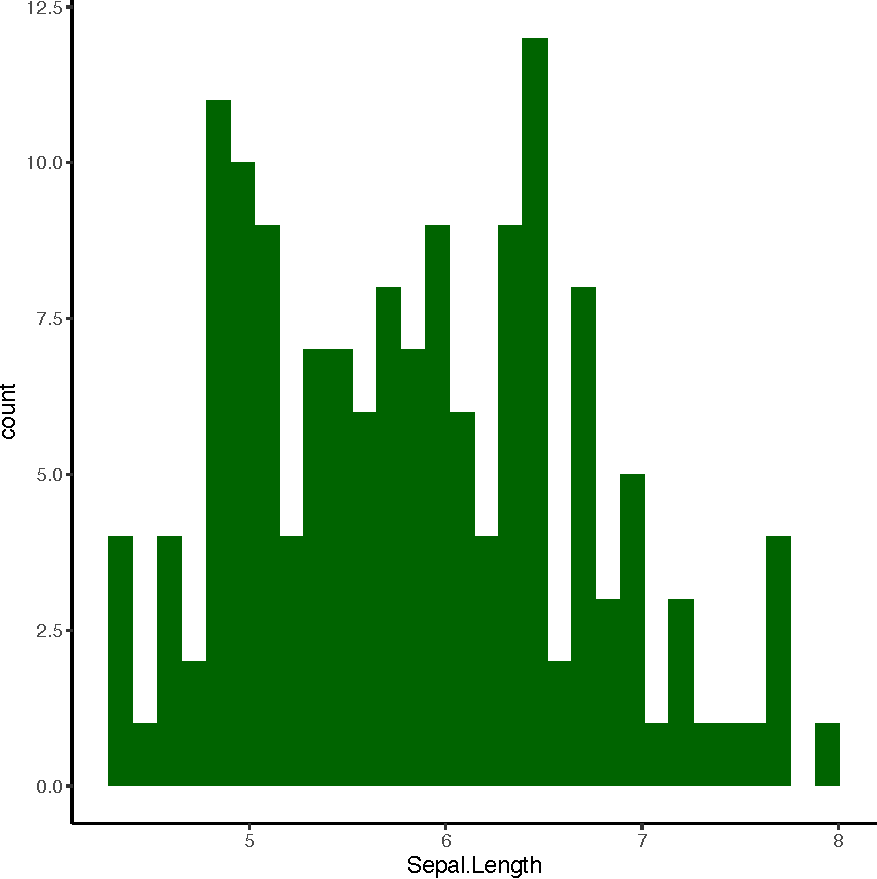
\includegraphics[width=0.8\linewidth]{/Users/cornelius/R_data/Rproject_template/output/reports/report_files/figure-latex/chunk with plot-1} \end{center}

\end{document}
